%!TEX root = ../thesis.tex

\chapter{Introduction}


%\ifpdf
 %   \graphicspath{{Chapters/Figs/Raster/}{Chapters/Figs/PDF/}{Chapters/Figs/}}
%\else
%    \graphicspath{{Chapters/Figs/Vector/}{Chapters/Figs/}}
%\fi


%********************************** % Section  **************************************
\section{Development Models}
\label{sec:devmodels}


Every industrial product has its own \textit{life-cycle} which starts when comes out the need of a new product and continues with the requirements identification, design, development and verification processes. Furthermore several other activities regarding the product maintenance could be as well part of the cycle. There are several approaches describing the sequentiality of product life cycle tasks, such as the so called \textit{Waterfall model} (Fig.\ref{fig:waterfall}), in which a phase starts after the completion of the previous one and phases' deliverables follows an unidirectional flows like in a pipeline.
\begin{figure}[!h]
	\centering 
     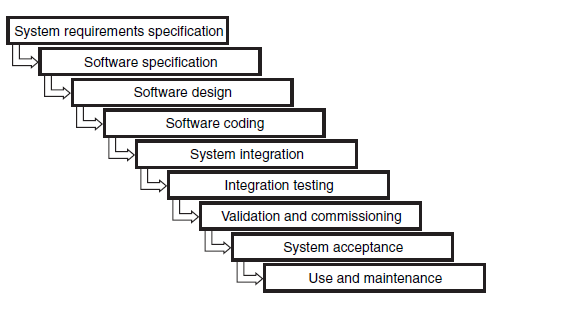
\includegraphics[width=.75\textwidth]{Figs/waterfall.png} 
     \caption{Waterfall Model} 
     \label{fig:waterfall} 
\end{figure} 

A example of the waterfall model we can examine the military standard MIL-STD-2167A, which establish a uniform development model applicable during the whole system life-cycle.
\par As second alternative  the \textit{V-model} (Fig.\ref{fig:vmodel}) enforces the temporal correlation among developing and validation phases. Activities on the left hand side of the V are associated with models of the system, where each subsequent activity represents an enhancement of the model from the previous activity. Processes on the right hand side of the V correspond to experimental (testing) activities. Results of a test phase validate the structure of the correspondent developing phase.

\begin{figure}[!h]
	\centering 
     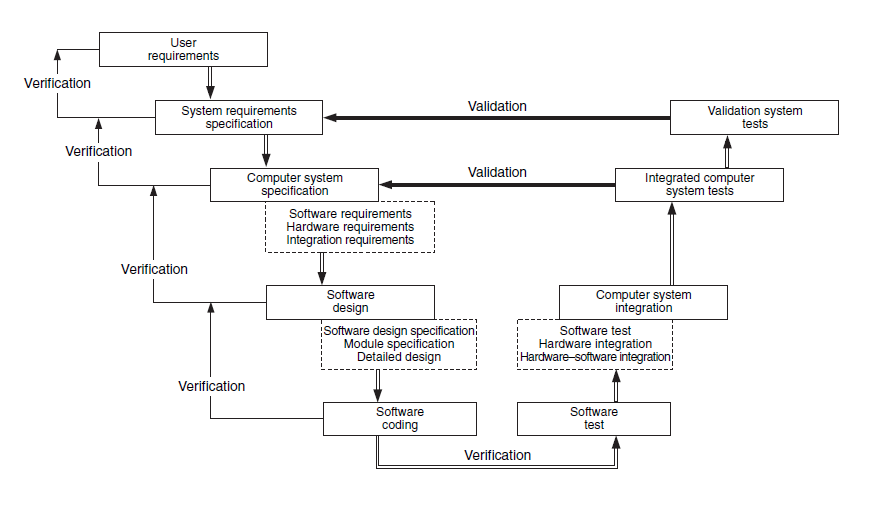
\includegraphics[width=\textwidth]{Figs/vmodel.png} 
     \caption{V-Model} 
     \label{fig:vmodel} 
\end{figure} 

This work focuses on the first stage of a generic product development model, i.e. Requirement analysis, trying to reduce the gap also with its relative validation.

%********************************** % Section  **************************************
\section{Requirements Fundamentals}
\subsection{Definition}
\begin{quote}
"...Requirements definition is a careful assessment of the needs that a system is to fulfill. It must say why a
system is needed, based on current and foreseen conditions, which may be internal operations or an external market. It must say what system features will serve and satisfy this context. And it must say h ow the
system is to be constructed..." — Doug Ross [Ross77a]
\end{quote}
Regardless of the adopted development model, the first, and critical, step to approach a product development is the System Requirement specification. It is much more than a functional specification, it is the groundwork for all the future stages and hence it has to catch everything is needed in terms of performance, behaviors and constraints to be satisfied. 
\par Being the requirement analysis the fundamental step that drives the design and implementation phases it is also worth noting how errors at this stage, \textit{late} errors, are much more costly in terms of time to be fixed than \textit{early} errors. The DoD Software Technology Plan \citep{DoD91} states that "early defect fixes are typically two orders of magnitude cheaper than late defect fixes, and the early requirements and design defects typically leave more serious operational consequences."

\subsection{Guidelines}


The result of the system requirements specification process is an
unambiguous and complete specification document. It should help:
\begin{enumerate}[label=\alph*)]
\item System customers to accurately describe what they wish to obtain;
\item System suppliers to understand exactly what the customer wants;
\end{enumerate}
Furthermore to the stakeholders a good system requirements specification (SRS) should provide several specific benefits, such as the following:
\begin{itemize}[label={--}]
\item \textit{Establish the basis for agreement between the customers and the suppliers on what the software
product is to do}. The complete description of the functions to be performed by the software specified
in the SRS will assist the potential users to determine if the software specified meets their needs or
how the software must be modified to meet their needs
\item \textit{Reduce the development effort}. The preparation of the SRS forces the various concerned groups in
the customer’s organization to consider rigorously all of the requirements before design begins and
reduces later redesign, recoding, and retesting. Careful review of the requirements in the SRS can
reveal omissions, misunderstandings, and inconsistencies early in the development cycle when these
problems are easier to correct.
\item \textit{Provide a baseline for validation and verification.} Organizations can develop their validation and
verification plans much more productively from a good SRS. As a part of the development contract,
the SRS provides a baseline against which compliance can be measured.
\end{itemize}
\par Attempts to reduce as much as possible the inconsistencies coming from the plain text descriptions has been proposed in several standards. The IEEE 830-1998 \citep{ieee1998ieee} offers a metric to produce and evaluate a good system requirements specification in terms of 
\begin{enumerate}[label=\alph*)]
\item Correctness
\item Unambiguity
\item Completeness
\item Consistency
\item Verifiability
\item Modifiability
\item Traceability
\end{enumerate}
while the MIL-STD-498 \citep{united1994mil} was a United States military standard whose purpose was to establish uniform requirements for systems development and documentation. Those standards rather than automatic tools are sort of guidelines to achieve a good specification for the system.

\subsection{Requirement Specification languages}
As said above, the requirement document quite often serves as a "contract" between designers and the costumers, as such it has to be somehow understandable also from those people having a non technical background, so quite often they are given with many pages of natural language descriptions, sometimes flanked with manually derived diagrams that represent the structure of the design. Due to its nature, the natural language specification of a property could be very far, and sometimes totally unrelated, from a formal definition. For instance natural language could be lacking, redundant or misleading, even worse the requirement definition is generally the result of an empirical process subjected to ambiguity, subjectivity and imprecisions.
\par The literature provides several methods aiming to avoid bad-formed requirements, all of them are based on the addition of a certain degree of formality in the syntax used to define the property referring a specific requirement. The most general classification of the specification languages is into \textit{formal}, \textit{semi-formal} and \textit{informal}.
\par A language is formal if its syntax and semantic are defined in a rigorous mathematical way. A formally expressed requirement provides an high level of verifiability, furthermore the process of translating natural into formal language requires the analysts to improve their comprehension of the requirement semantic. In fact, in order for the translation to be successful they have to verify, and eventually eliminate, the presence of ambiguities also from the natural language definition.
\par Semi-formal languages are usually expressed in a graphical manner, aimed to provide a non-ambiguous description through a generally easier syntax that has not a direct mapping to a mathematical semantic. The \textit{structured natural language}, which will be of interest in below discussions, could be in turn part of this category. In particular it could be view as a plain text which has some constraint in the precedence of sentences participants.%ref to UML-SysML??
\par Informal languages are those that have neither a rigorous syntax or rigorous semantic. In particular the syntax is derived from the relative grammatic and the semantic is that rich that makes impossible its formalization. Despite all this, they are the most commonly used, and, hence, a good specification always relies on the experience of designers.

\subsection{Readability versus Formality}
The more we increase the syntax formality and the more the number of possible inconsistencies is reduced. As drawback requirement specification starts taking a non-easy readable shape and becomes very distant from its natural language expression. There are several reasons why this aspect represents an obstacle to the usability of these techniques. First, a requirements document could not be anymore used as sort of contract among stakeholders since there are no guarantees that one of the parts is able to understand the meaning of the formula. Further, their use implies engineer to have a certain level of expertise in typing formal requirements. Although the usability does not constitute the strength of this approach the reason why formal languages are still of interest is due to their capability of totally avoid formulas ambiguity.

\subsection{Requirements Specialization}
A direct consequence of the use of formal languages is the possibility to perform automatic verification techniques out of the requirements, but, as previously said, rarely the specifications are formally written, implying, hence, several manual translation stages from natural language. 
\par This work bridges the gap between formal and informal representation of requirements. In order to do so the effort has been spread along an ideal line starting from the natural up to the formal language description. The first step consists of defining a syntax which allows the presence of free-text, limited to certain points of the sentence, and, at the same time, preserves a well defined structure. Once the requirements are structured is then possible to apply some processing technique able to recognize every \textit{common pattern}, i.e. all those properties having a direct correlation, in terms of temporality or property semantic, with a specific formal language pattern. Finally the formal properties are used to generate automatically verification monitors.
\begin{figure}[!h]
	\centering 
     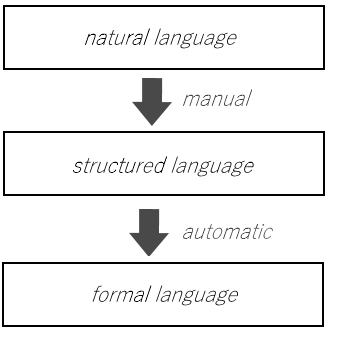
\includegraphics[width=.4\textwidth]{Figs/specialization.png} 
     \caption{Requirement specialization} 
     \label{fig:reqspec} 
\end{figure} 
 
\subsection{High-Level Requirements}
Rarely system requirements are written in a formal language, the non-rigorous nature of plain text constitutes the main obstacle to automatic generation of monitors out of the specification. Writing requirements in a semi-formal shape rather than a plain text will make them suitable to language processing techniques which allow to get their formal specification. As enforcement of this concept, in certain specific application domain requirements usually refer to properties having a well-known semantic. Typically for such cases also plain text requirements tend to have a fixed structure. This scenario commonly recurs when the specification is given from an high level of abstraction of the systems and, hence, does not regard constraints on the development. Performance requirements in a control system are an example. In fact they have an invariant textual form compared, for instance, to system's hardware structure or control algorithms.
%********************************** % Section  **************************************
\section{Verification tools}

\subsection{Property checking}

In general, the problem of determining whether a property $\phi$ is satisfied from system $S$ could be faced in many ways depending on the set of environmental conditions in which system and property are defined. Being not too much formal we can define a system $S$ as an entity that correlates inputs and output signals according to a precise law, while the \textit{model} of the system as a set of possible \textit{states} in which system can lie, each state $x_{i}$ ranging over the domain $X_{i}$. A system evolves over the time domain and the function $\beta :T\rightarrow X$, associating a state to a precise time instant, is called \textit{behavior} of the systems. 
Within this context a property $\phi$ defines a subset of the systems' state and a property \textit{monitor} is that entity that ensures whether a certain behavior \textit{satisfies} the property, i.e. whether $L_{\phi}\in X$.
\par The procedure leading to the verification of a property, or formula, consists of associating a function $\Omega_{\phi}:X\rightarrow B$ which, given the set of all possible behaviors returns a boolean value meaning whether the property is satisfied or not. Behaviors are examined one at time assuming the presence of a simulation unit charged to produce them. 
A monitor is hence another unit which cooperates with the system simulator mainly in three ways (Fig.\ref{fig:monitortypes}). 

\begin{figure}[!h]
	\centering 
     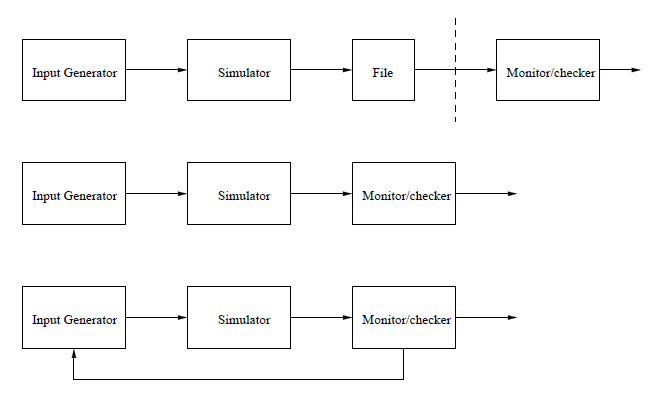
\includegraphics[width=.8\textwidth]{Figs/monitortypes.png} 
     \caption{Off-line, Passive On-line and Active On-line monitors from \citep{maler2008checking}} 
     \label{fig:monitortypes} 
\end{figure} 
The \textit{off-line} monitoring expects monitors to check formulas against the simulation traces. Since monitors are no forced to be causal over the execution time this technique constitutes the easiest way to conduce model checking. In the \textit{on-line} methods the monitor is running in parallel with the simulator, we refer to \textit{active} on-line if the monitor is also affecting, through a feed-back loop, the simulation inputs, and \textit{passive} on-line otherwise. In general on-line monitors have the advantage of being able to assert satisfaction or violation of a property while the simulation is running, this prevents either high time consuming simulation to be terminated and dangerous behavior to occur after the violation of the property. The cost we pay for an on-line monitoring is that formulas must be causal, i.e. it is not possible to check a property at certain time $t$ as function of states occurring later than $t$. Since this work focuses mostly on dynamic controls system domain monitors that are better suited to fit it are of the type passive on-line. 

\subsection{Automatic monitor generation}
Under the assumption that requirements are written in formal language, i.e. absence of inconsistencies, the generation of verification monitors for simulation can be performed in an automatic way. 
\par Code generation procedures are always targeted to a specific platform, which in turn varies as function of the application domain. For what regards dynamical systems typical targets are simulation frameworks such as Simulink by Matworks\citep{Simulink} and LabVIEW\citep{Labview}. Together with the target platform usually code generation starts from a model of the entities we want generate for. 
\par Tools such as Acceleo\citep{acceleo} are based on the prior definition of the mode of the system architecture, allowing language independent code generation from any kind of EMF compatible meta-model, such as UML, UML 2.0 and SysML. Also Simulink with the Embedded Coder offers the possibility to customize the C/C++ code generated from any Simulink model.
\par Another chance is to not rely on the presence of a system model and generate code implementing verification monitors directly from statements expressed in some formal language. The work in \citep{bals2017} starts from properties expressed in the STL formal language\citep{maler2008checking} and produces Simulink monitors, to ease the auto-generation procedure it makes use of a library implementing the STL temporal operators.

\section{Proposed Tool}

\subsection{Premise}
This work aims to show the feasibility of a tool that starts from semi-formal system specification and ends up with verification monitors to be plugged into a simulation model of the system. The number of particular cases to deal with it is huge and the scalability of the approach is a key factor that needs time to be proved. However, due to the impact that such a tool could have in the design and verification processes, the problem has been sized in order to be manageable at least with the purpose of producing a proof of concept prototype.
\par For the above reasons we decide to use, as a case study, the high-level requirements for dynamic control systems. Such requirements has been restructured in the \textit{contract-base} paradigm, which, basically, expect the formulation of the property as a composition of two main sections, \textit{assumption} and \textit{assertion}, were the first logically implies the second.
\par Further the formalization of the requirements has been performed using the STL formal language, which, unlike many others temporal logics derived from LTL, adds some domain specific features that will be better described in sec.\ref{sec:STL}. Finally, as target platform, Simulink has been selected since it is one of the most used simulation tools for such application domain. A graphical representation of the whole framework together with the smart editor, which will be discussed in next section, is presented in figure \ref{fig:framework}.

\begin{figure}[!h]
	\centering 
     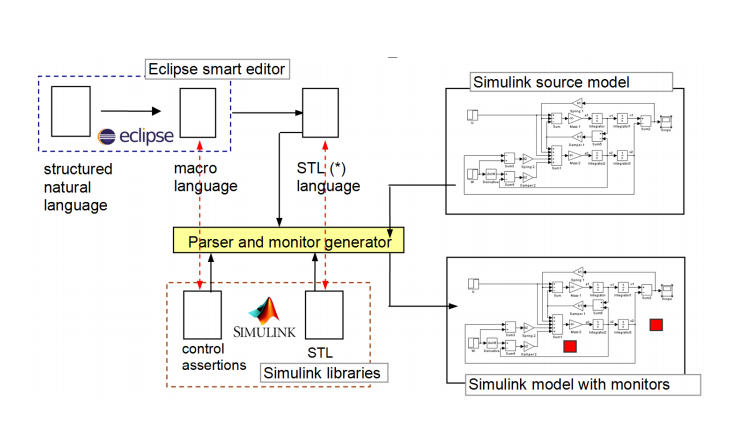
\includegraphics[width=1\textwidth]{Figs/framework.png} 
     \caption{Framework} 
     \label{fig:framework} 
\end{figure}

\subsection{Custom Editor}
The smart editor is meant as the tool helping users to write semi-formal requirements. It has been implemented as an Eclipse Editor plug-in, from which inherits many features common to most commercial editors such as \textit{context-aware} text completion and syntax error checking. The editor comes with it is own syntax which even if for the time being is deeply application domain oriented preserves a modular an easily extensible software structure.
\par Some more specific features are the capability to import a data dictionary which is ideally synchronized with the target model and generate platform dependent monitors. 